\documentclass[12pt,a4paper]{report}

\usepackage[utf8]{inputenc}
\usepackage[czech]{babel}
\usepackage[T1]{fontenc}
\usepackage{geometry}
\usepackage{microtype}
\geometry{margin=2.5cm}
\usepackage[hidelinks]{hyperref}
\usepackage{graphicx}
\usepackage{subcaption}
\usepackage{placeins}
\usepackage{float}
\usepackage{etoolbox}
\makeatletter
\patchcmd{\@makechapterhead}{\vspace*{50\p@}}{\vspace*{0pt}}{}{}
\patchcmd{\@makechapterhead}{\vskip 40\p@}{\vskip 10pt}{}{}
\makeatother

\usepackage{listings}
\usepackage{xcolor}

\definecolor{codegray}{rgb}{0.5,0.5,0.5}
\definecolor{backcolour}{rgb}{0.95,0.95,0.92}

\lstset{
    backgroundcolor=\color{backcolour},
    commentstyle=\color{green!60!black},
    keywordstyle=\color{magenta},
    numberstyle=\tiny\color{codegray},
    stringstyle=\color{orange},
    basicstyle=\ttfamily\small,
    breakatwhitespace=false,
    breaklines=true,
    captionpos=b,
    keepspaces=true,
    numbers=left,
    showspaces=false,
    showstringspaces=false,
    showtabs=false,
    tabsize=2,
    language=Python
}


\begin{document}
\begin{titlepage}
   \centering
 
    
\includegraphics[width=0.4\textwidth]{img/zcu_logo.png} \\ 
    \vspace{1cm}
    
    \Huge
    \textbf{3D Laserový Skener} \\
    \vspace{0.5cm}
    \Large
    Projekt Raspberry Pi 5 \\
    \vspace{1cm}
    \large
    Technická dokumentace
    
    \vfill
    
    \large
    \textbf{Autoři} \\
    \vspace{0.5cm}
    \begin{tabular}{cc}
        	\textbf{Eduard Štich}  & Jan Pilař \\
	Daniel Otta  &  Václav Dubský\\
        	Hynek Lávička   &  Lukáš Riedl\\      
      	 Petr Špaček  &  Dominik Hebeda \\
	 Patrik Janovec &  Jakub Husák  \\
    \end{tabular}

    \vfill
    \today

\end{titlepage}

\setcounter{page}{2}
\tableofcontents
\clearpage

\chapter{Specifikace projektu}

Cílem projektu je návrh a realizace cenově dostupného 3D skeneru. Projekt reaguje na \mbox{vysokou} pořizovací cenu profesionálních technologií a představuje efektivní řešení  \mbox{postavené} na platformě Raspberry Pi 5.

\section{Účel a motivace}
Zařízení slouží k automatizované digitalizaci menších objektů. Hlavním přínosem \mbox{našeho} řešení je  demokratizace složité technologie 3D skenování. Využitím osvědčené metody laserové \mbox{triangulace} dosahujeme  výrazného snížení nákladů při zachování technické kvality výstupu v podobě mračna bodů.

\section{Technické řešení}
Jádrem systému je mikropočítač Raspberry Pi 5, který zajišťuje koordinaci dvou liniových laserů a dvou Pi kamer, přesné polohování objektu pomocí krokového motoru a obsluhu webového rozhraní pro vzdálenou správu.

\section{Parametry zařízení}
\begin{table}[h]
    \centering
    \begin{tabular}{|l|l|}
        \hline
        \textbf{Parametr} & \textbf{Hodnota} \\ \hline
        Řídicí jednotka & Raspberry Pi 5 \\ \hline
        Metoda snímání & Laserová triangulace \\ \hline
        Snímací hardware & 2$\times$ Pi kamera, 2$\times$ Liniový laser \\ \hline
        Rozsah rotace & 360° (krokový motor) \\ \hline
        Náklady & $\approx$ 1\,800~Kč \\ \hline
    \end{tabular}
    \caption{Základní technická specifikace skeneru}
\end{table}

\section{Konstrukční cíle}
Důraz je kladen na uzavřené provedení konstrukce, které eliminuje externí světelný šum a zajišťuje mechanickou stabilitu všech měřicích komponent vůči ose rotace.

\chapter{Princip 3D skenování}
Základním principem fungování tohoto zařízení je metoda laserové triangulace. Tato \mbox{technika} využívá známé geometrické vztahy mezi zdrojem světla, snímačem a měřeným objektem k určení přesných souřadnic bodů v trojrozměrném prostoru.

\section{Princip laserové triangulace}
Celý proces je založen na vytvoření pomyslného trojúhelníku, jehož vrcholy tvoří čočka kamery (v tomto případě Pi kamer), zdroj laseru a bod na povrchu skenovaného objektu. 

\begin{itemize}
    \item \textbf{Projekce linie:} Liniový laser vysílá úzký paprsek světla, který po dopadu na objekt vytvoří světelný řez jeho povrchem. 
    \item \textbf{Snímání deformace:} Kamera, která je vůči laseru umístěna pod pevným úhlem, snímá tuto linii. Pokud je povrch objektu rovný, jeví se linie jako přímka. Jakmile však narazí na reliéf, linie se z pohledu kamery v horizontální rovině deformuje.
    \item \textbf{Výpočet souřadnic:} Software analyzuje horizontální posun každého pixelu \mbox{laserové} čáry v obraze. Čím blíže je povrch objektu ke kameře, tím více je čára vychýlena do strany. Pomocí goniometrických funkcí a znalosti tzv. \textit{báze} (pevná vzdálenost mezi laserem a kamerou) lze vypočítat přesnou hloubku každého bodu.
\end{itemize}



\section{Metoda rotačního skenování}
Aby bylo možné získat kompletní 360° model objektu, je skener vybaven otočnou \mbox{platformou}, což umožňuje nasnímat objekt ze všech stran bez nutnosti manipulace se zdrojem světla nebo kamerami.

\begin{itemize}
    \item \textbf{Krokový motor:} Zajišťuje rotaci podstavce o přesně definované úhly. Každý krok motoru představuje nový vertikální řez objektem.
    \item \textbf{Sekvenční snímání:} Po každém pootočení proběhne nová expozice a výpočet \mbox{profilu.} 
    \item \textbf{Mračno bodů (Point Cloud):} Výsledkem procesu je soubor tisíců bodů se souřadnicemi $[X, Y, Z]$. Tyto body dohromady tvoří digitální otisk povrchu, který lze následně v postprocessingu převést na polygonální síť (mesh).
\end{itemize}
\chapter{Konstrukce a vývoj krabice}
Krabice skeneru je navržena jako uzavřený box o vnějších rozměrech 24 × 18 × 15 cm. Tato velikost byla zvolena jako ideální kompromis mezi kompaktností a schopností \mbox{skenovat} \mbox{objekty} běžné velikosti ($\approx$ do 10 cm výšky). Konstrukce vychází z konceptu Raspberry Pi Laser Scanner [1], oproti kterému však bylo zvoleno robustnější řešení.\\\\
Hlavním důvodem pro toto uzavřené řešení je zajištění stálých světelných podmínek uvnitř skeneru. Vnější světlo by mohlo negativně ovlivňovat přesnost laserových linií při snímání Pi kamerami. Pevné stěny krabice navíc pomáhají tlumit vibrace od motoru, což zabraňuje rozmazání výsledného 3D modelu. Růžové body v modelu znázorňují pozice pro umístění skenovacích prvků.
\begin{figure}[h]
    \centering
   
    \begin{subfigure}[t]{0.45\textwidth}
        \centering
	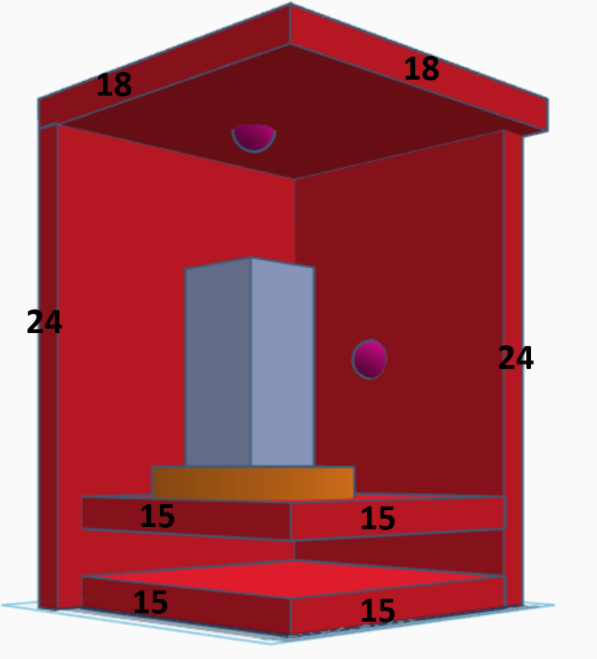
\includegraphics[width=\textwidth]{img/krabice_rozmery.png} 
        \caption{Čelní pohled}
    \end{subfigure}
    \hfill
   \begin{subfigure}[t]{0.45\textwidth}
        \centering
        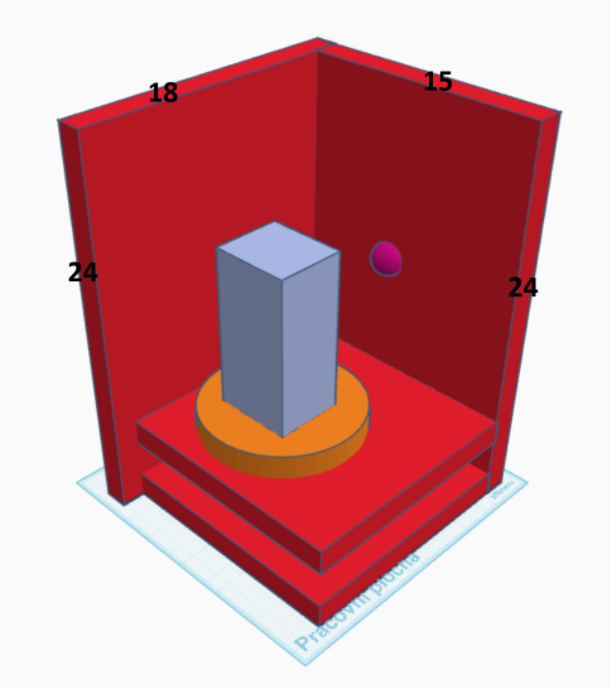
\includegraphics[width=\textwidth]{img/krabice_vnitrek.png}
        \caption{Perspektivní pohled}
    \end{subfigure}
\caption{Technické nákresy a vizualizace konstrukce krabice}
\end{figure}

\chapter{Hardwarová část}
\section{Tištěné specifické díly}
Jednotlivé mechanické díly byly navrženy tak, aby bylo dosaženo přesného ustavení \mbox{optických} i pohonných prvků konstrukce. Držáky laserů společně s držákem motoru \mbox{zajišťují} tuhost sestavy, která je klíčová pro eliminaci geometrických odchylek během rotace snímaného objektu. Tvary i rozměry těchto komponent byly optimalizovány pro technologii 3D~tisku, čímž bylo dosaženo nízké hmotnosti při zachování vysoké pevnosti dílů.\\\\
Důležitou součástí jsou také krytky s vývody pro kabeláž, které slouží k organizaci  \mbox{vodičů} a zabraňují jejich nechtěnému kontaktu s pohyblivými částmi skeneru. Variabilita v   \mbox{provedení} krytek umožňuje flexibilní vedení tras k řídicí jednotce bez nutnosti ostrých ohybů kabelů.
\begin{figure}[H]
    \centering
    % 1. řada
    \begin{subfigure}[t]{0.45\textwidth}
        \centering
        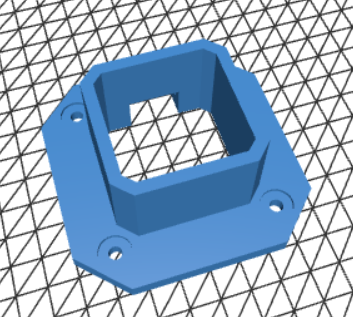
\includegraphics[height=3.5cm,keepaspectratio]{img/motor.png}
        \caption{Držák krokového motoru}
    \end{subfigure}
    \hfill
    \begin{subfigure}[t]{0.45\textwidth}
        \centering
        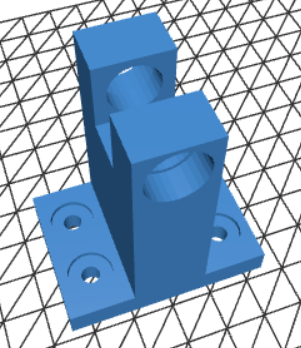
\includegraphics[height=3.5cm,keepaspectratio]{img/laser_hor.png}
        \caption{Horizontální držák laseru}
    \end{subfigure}
\vspace{0.3cm}
    % 2. řada
    \begin{subfigure}[t]{0.45\textwidth}
        \centering
        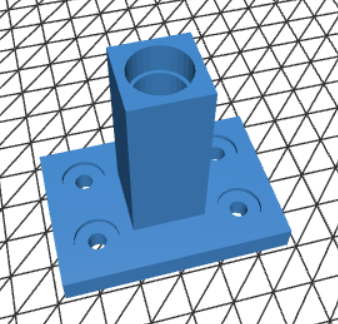
\includegraphics[height=3.5cm,keepaspectratio]{img/laser_ver.png}
        \caption{Vertikální držák laseru}
    \end{subfigure}
    \hfill
    \begin{subfigure}[t]{0.45\textwidth}
        \centering
        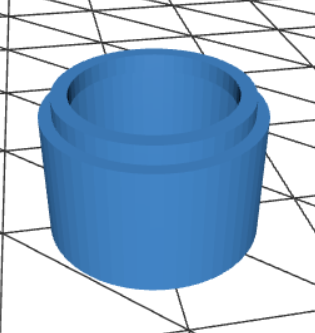
\includegraphics[height=3.5cm,keepaspectratio]{img/krytka_laser_hor.png}
        \caption{Krytka laseru}
    \end{subfigure}
 \vspace{0.3cm}
     % 3. Řada
    \begin{subfigure}[t]{0.45\textwidth}
        \centering
        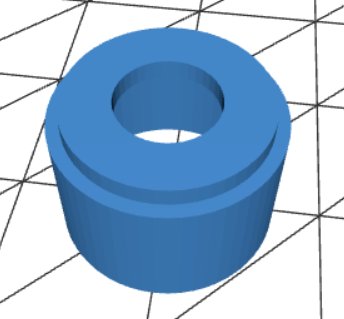
\includegraphics[height=3.5cm,keepaspectratio]{img/krytka_laser_hor_kabely.png}
        \caption{Krytka s vývodem (horizontální)}
    \end{subfigure}
    \hfill
    \begin{subfigure}[t]{0.45\textwidth}
        \centering
        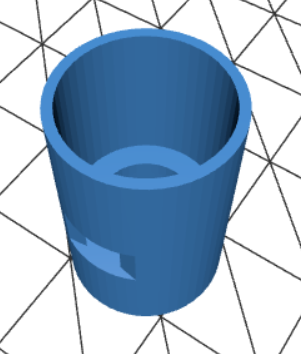
\includegraphics[height=3.5cm,keepaspectratio]{img/krytka_laser_ver_kabely.png}
        \caption{Krytka s vývodem (vertikální)}
    \end{subfigure}
    
    \caption{Detailní přehled 3D modelů specifických dílů hardwaru.}
\end{figure}
\FloatBarrier
\section{Seznam komponent}
Skladba komponent byla zvolena s ohledem na dosažení nízkonákladového řešení ($\approx$~1\,800\,Kč) při zachování vysoké přesnosti měření.

\begin{itemize}
    \item \textbf{Řídicí jednotka:} Raspberry Pi 5
    \item \textbf{Snímací hardware:}
    \begin{itemize}
        \item 2$\times$ Pi kamera (kamerový modul v2, 8\,Mpx)
        \item MIPI FFC flex video kabel (50 cm) pro flexibilní umístění Pi kamer
        \item 2$\times$ Liniový laserový modul (červený, 5\,V, 5\,mW, 650\,nm)
    \end{itemize}
    \item \textbf{Pohonný systém:}
    \begin{itemize}
        \item Krokový motor NEMA 17 (17HS3401, 0.28\,Nm)
        \item A4988 driver pro přesné řízení kroků motoru
    \end{itemize}
    \item \textbf{Elektronika a UI:}
    \begin{itemize}
        \item LCD displej s I2C rozhraním
        \item Nepájivé pole (400 bodů) pro realizaci spojnicové desky
        \item Silikonový mikrospínač (8x8x5\,mm) pro manuální ovládání
        \item Sada rezistorů
    \end{itemize}
    \item \textbf{Konstrukční díly:} Specifické 3D tištěné držáky a krytky
\end{itemize}
\clearpage
\section{Schéma zapojení}
Propojení všech elektronických komponent je realizováno prostřednictvím nepájivého pole, které slouží jako centrální uzel pro distribuci napájení i~datových signálů. Celkové schéma zapojení vytvořené v~prostředí Fritzing je znázorněno na obrázku \ref{fig:schema}.

\begin{figure}[h]
    \centering
    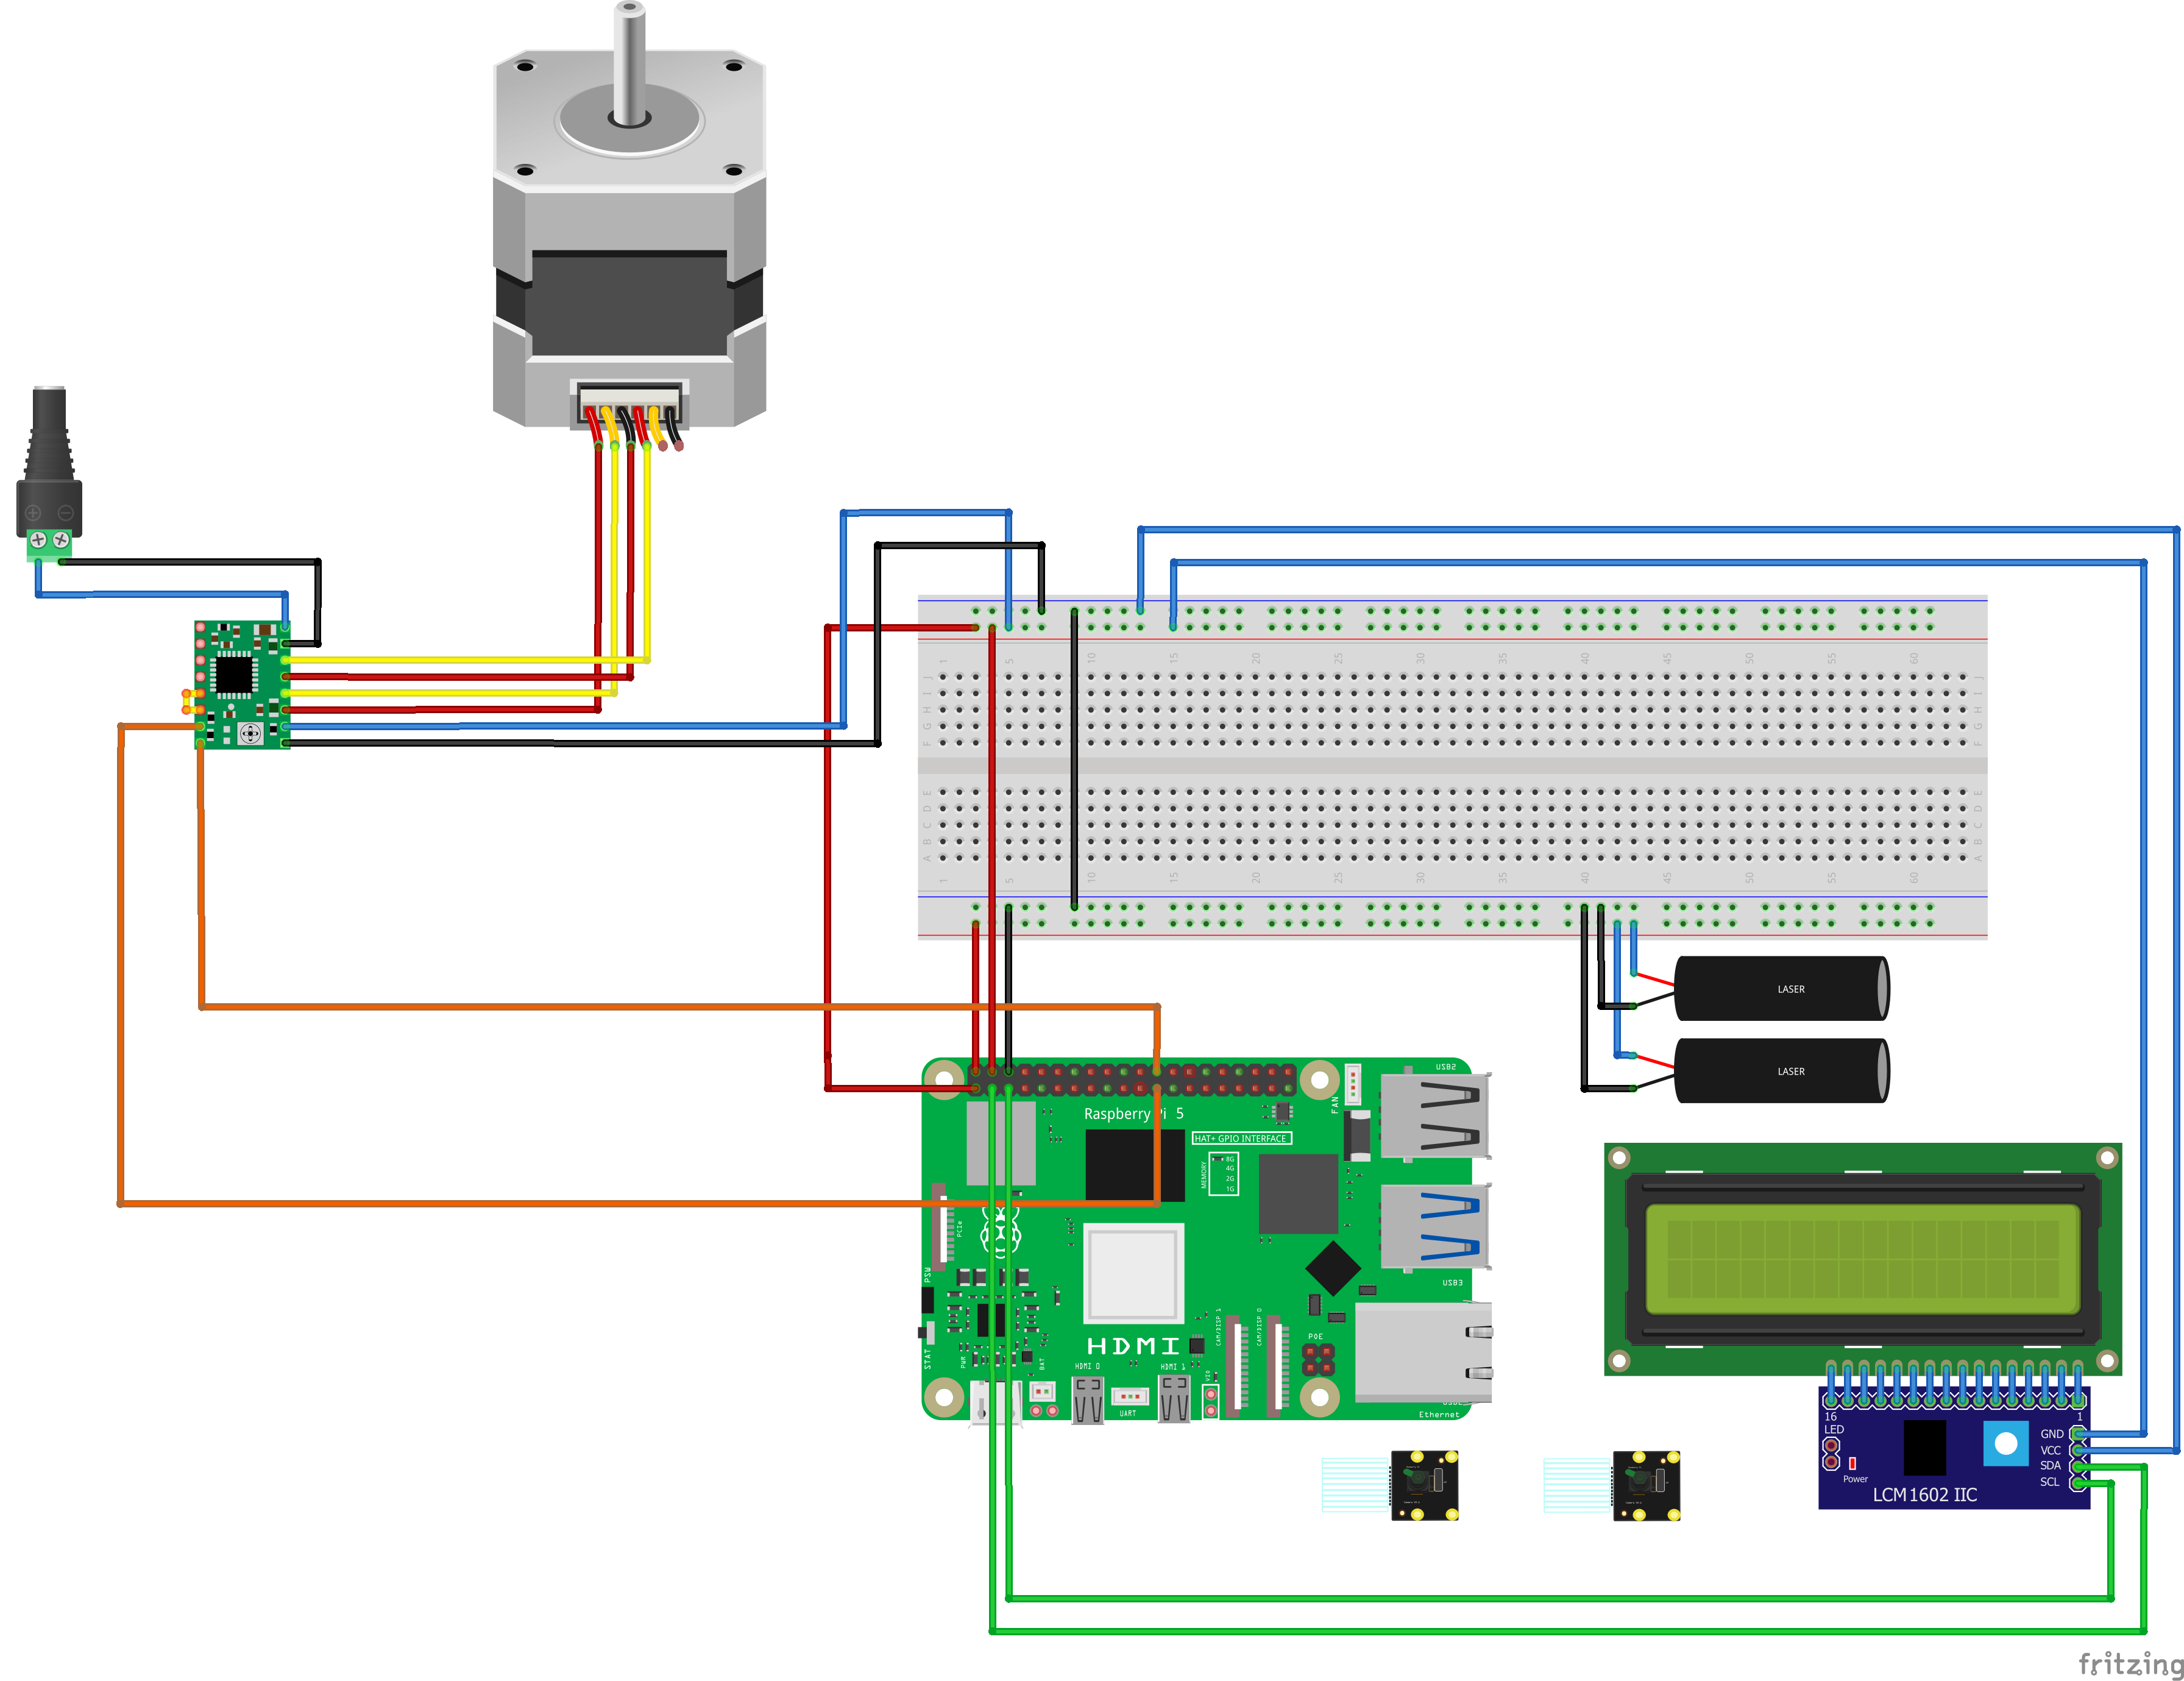
\includegraphics[width=0.9\textwidth]{img/schema_zapojeni.png}
    \caption{Kompletní schéma zapojení 3D skeneru}
    \label{fig:schema}
\end{figure}
\clearpage
\subsection{Detailní zapojení komponent}
Následující tabulky specifikují propojení jednotlivých prvků s~řídicí jednotkou Raspberry Pi 5 a externím napájením.

\begin{table}[H]
    \centering
    \begin{tabular}{|l|l|p{7cm}|}
        \hline
        \textbf{Driver A4988} & \textbf{Cílový pin / Zdroj} & \textbf{Funkce a poznámka} \\ \hline
        VMOT & Externí zdroj (12\,V) & Přívod hlavního proudu pro pohon \mbox{samotného} motoru. \\ \hline
        GND (napájení motoru) & Externí zdroj (GND) & Uzemnění externího zdroje. Propojeno s~GND Raspberry Pi. \\ \hline
        1A, 1B / 2A, 2B & Cívky motoru & Výstupy napájející přímo první \mbox{a druhou} cívku motoru. \\ \hline
        VDD / GND & RPi Pin 1 / Pin 6 & Napájení logiky driveru (3,3\,V) \mbox{a společné} uzemnění. \\ \hline
        STEP & RPi Pin 23 (GPIO 11) & Přijímá pulzy z~RPi (každý přechod 1-0 vykoná jeden krok). \\ \hline
        DIR & RPi Pin 24 (GPIO 8) & Logická úroveň určuje směr otáčení \mbox{(závislé} na zapojení motoru). \\ \hline
        RST / SLP & Vzájemné propojení & Piny jsou propojeny mezi sebou, čímž je driver trvale aktivní. \\ \hline
    \end{tabular}
    \caption{Detailní zapojení driveru A4988 pro řízení krokového motoru}
\end{table}

\begin{table}[H]
    \centering
    \begin{tabular}{|l|l|p{7cm}|}
        \hline
        \textbf{Periferie} & \textbf{Zapojení (RPi)} & \textbf{Funkce a poznámka} \\ \hline
        Kamerové moduly & CSI port 0 a 1 & Snímání obrazu (dolní a horní kamera) přes sběrnici CSI. \\ \hline
        Liniové lasery & Pin 2 (5\,V) / Pin 6 & Napájení laserů a uzemnění přes \mbox{breadboard}. \\ \hline
        LCD VCC / GND & Pin 1 (3,3\,V) / Pin 6 & Napájení I2C modulu a displeje se \mbox{společnou} zemí. \\ \hline
        LCD SDA & Pin 3 (SDA) & Datová linka I2C sběrnice pro \mbox{komunikaci} s~displejem. \\ \hline
        LCD SCL & Pin 5 (SCL) & Hodinový signál I2C sběrnice \mbox{generovaný} Raspberry Pi. \\ \hline
    \end{tabular}
    \caption{Zapojení kamer, laserů a informačního displeje}
\end{table}

\textit{Poznámka: Pro správnou funkci logických signálů jsou všechny záporné póly (GND) z~Raspberry Pi, externího zdroje i~periferií vzájemně propojeny na společnou sběrnici nepájivého pole.}

\chapter{Softwarová část a nastavení RPi}

\section{Instalace OS a základní konfigurace}
Pro řízení skeneru byl zvolen mikropočítač Raspberry Pi 5. Jako operační systém byla použita distribuce \textbf{Raspberry Pi OS Lite (64-bit)}, která neobsahuje grafické rozhraní, což snižuje systémovou režii a zvyšuje stabilitu aplikací běžících na pozadí.

Při prvotní instalaci pomocí nástroje Raspberry Pi Imager byly nastaveny následující parametry pro vzdálený přístup a síťovou konektivitu:

\begin{itemize}
    \item \textbf{Hostname:} \texttt{skener.local}
    \item \textbf{Uživatelský účet:} 
    \begin{itemize}
        \item Jméno: \texttt{appuser}
        \item Heslo: \texttt{appuser}
    \end{itemize}
    \item \textbf{Vzdálený přístup:} Aktivováno SSH (Secure Shell) pro správu přes terminál.
    \item \textbf{Bezdrátové připojení:} Automatické připojení k síti (SSID: \texttt{zpp-rpi}).
\end{itemize}

\section{Instalace softwarových balíčků}
Po úspěšné instalaci systému a aktualizaci repozitářů byly doinstalovány klíčové \mbox{komponenty} nezbytné pro běh API a webového rozhraní. Správa balíčků probíhá standardně přes nástroj \texttt{apt}.

\begin{itemize}
    \item \textbf{Python:} Primární programovací jazyk pro logiku skenování, ovládání GPIO pinů (motory, lasery) a zpracování obrazu.
    \item \textbf{UFW (Uncomplicated Firewall):} Nástroj pro správu síťového provozu. Slouží k zabezpečení zařízení povolením pouze nezbytných portů (např. 22 pro SSH a 80 pro HTTP provoz).
\end{itemize}
\section{Nastavení potřebných služeb}
Pro zajištění autonomního běhu skeneru jsou klíčové procesy nastaveny jako systémové služby (\textit{systemd units}). To zajišťuje automatický start po zapojení napájení a automatický restart v případě chyby.
\begin{itemize}
    \item \textbf{scanner\_api.service:} Zajišťuje běh Flask/FastAPI serveru pro komunikaci s webem.
    \item \textbf{display\_handler.service:} Samostatný proces obsluhující I2C LCD displej.
\end{itemize}
\section{Simulace a generování testovacích dat}
Vzhledem k paralelnímu vývoji hardwaru a softwaru byla vytvořena virtuální simulace skeneru v prostředí Blender. Tento přístup umožnil vývoj algoritmů pro zpracování obrazu nezávisle na fyzické kompletaci zařízení.

\begin{figure}[H]
    \centering
    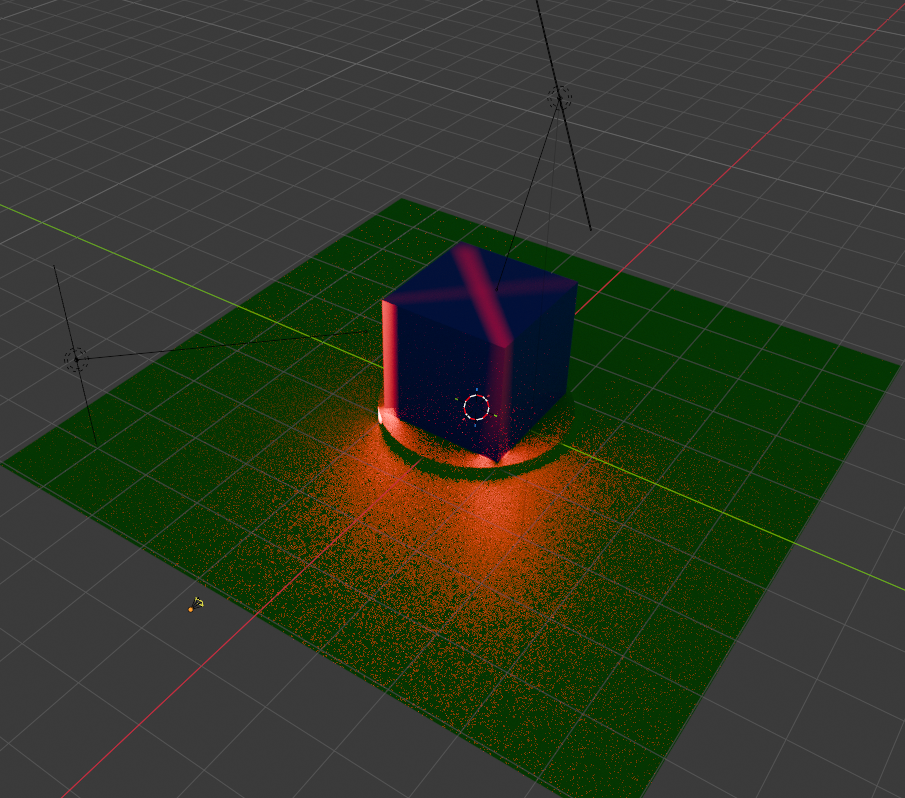
\includegraphics[width=0.85\textwidth]{img/blender_rendered.png}
    \caption{Renderovaná simulace skenovací scény: \textbf{modře} je vyznačen testovací objekt, \textbf{červeně} dopadající laserová linie, \textbf{zeleně} rotační podložka a \textbf{černě} jsou naznačeny směrové vektory kamer.}
    \label{fig:blender_render}
\end{figure}

Pro simulaci byl navržen virtuální setup odpovídající reálné konstrukci:
\begin{itemize}
    \item \textbf{Virtuální senzory:} Pozice kamer a liniových laserů přesně odpovídá geometrii krabice.
    \item \textbf{Datová sada:} Byla vygenerována sekvence minimálně 120 snímků rozložených rovnoměrně v rozsahu 360° rotace objektu.
    \item \textbf{Kvalita výstupu:} Snímky jsou renderovány v nativním rozlišení Pi kamer ($3280 \times 2464$\,px) bez externích zdrojů světla, což věrně simuluje podmínky uvnitř uzavřené konstrukce.
\end{itemize}
\clearpage
\section{Algoritmus zpracování obrazu a 3D rekonstrukce}
Jádrem softwaru je proces transformace 2D obrazových dat z Pi kamer do 3D mračna bodů. Tento proces probíhá v několika krocích.

\subsection{Detekce laserové linie pomocí HSV maskování}
Pro filtraci červeného laseru v obraze je využita segmentace v barevném prostoru HSV. Na rozdíl od RGB je HSV prostor méně náchylný na změny intenzity osvětlení.
\begin{lstlisting}[caption=Výstřižek kódu pro extrakci červených bodů]
hsv = cv2.cvtColor(img, cv2.COLOR_BGR2HSV)
lower_red1 = np.array([0, 150, 50])
upper_red1 = np.array([10, 255, 255])
mask = cv2.inRange(hsv, lower_red1, upper_red1)
mask = cv2.morphologyEx(mask, cv2.MORPH_OPEN, kernel)
\end{lstlisting}

\subsection{Matematický model rekonstrukce}
Každý nalezený bod v masce představuje průsečík laserové roviny a povrchu objektu. Výpočet souřadnice $Z$ (vzdálenost) a následný převod na kartézské souřadnice $[x, y, z]$ probíhá podle vztahů:
\begin{equation}
    x = radius \cdot \cos(\alpha) + offset_x
\end{equation}
\begin{equation}
    y = radius \cdot \sin(\alpha)
\end{equation}
\begin{equation}
    z = camera\_distance - \Delta y \cdot scale
\end{equation}
kde $\alpha$ odpovídá aktuálnímu kroku motoru převedenému na radiány.

\subsection{Tvorba polygonální sítě (Mesh)}
Mračno bodů je pomocí knihovny \texttt{trimesh} převedeno na výsledný model. Pro uzavření povrchu je využit algoritmus \textit{Convex Hull}. Software dále podporuje booleovské operace (rozdíl modelů), které umožňují odečíst referenční model podložky od výsledného skenu objektu.
\chapter{Uživatelské rozhraní}
Tato kapitola popisuje způsoby interakce uživatele se skenerem. Zařízení kombinuje \mbox{vzdálenou} správu pomocí webové aplikace pro plnou kontrolu nad procesem a lokální informační displej pro okamžitou diagnostiku stavu.

\section{Webové rozhraní}
Uživatelské rozhraní je navrženo jako responzivní webová aplikace založená na standardech HTML5 a JavaScriptu. Aplikace (Dashboard) komunikuje asynchronně s~API běžícím na Raspberry Pi 5, což umožňuje plynulé ovládání bez nutnosti obnovování stránky.

\begin{itemize}
    \item \textbf{Hlavní ovládací panel:} Obsahuje prvky pro spuštění skenování (\textit{Start}), pozastavení (\textit{Stop}) a nouzové ukončení procesů (\textit{Kill}).
    \item \textbf{Indikace průběhu:} Dynamický progress bar zobrazuje aktuální stav skenování v procentech na základě dat ze stavového boxu.
    \item \textbf{Správa skenů:} Sekce pro prohlížení a stahování hotových 3D modelů ve formátu .STL.
\end{itemize}

\section{Informační displej}
Pro okamžitou vizuální zpětnou vazbu bez nutnosti kontroly webového rozhraní je zařízení osazeno LCD displejem $16\times2$ znaků s I2C sběrnicí. Displej slouží jako stavový indikátor, který v reálném čase interpretuje data přijímaná z hlavní řídicí aplikace.

\subsection{Logika zobrazení a stavový automat}
Program obsluhující displej pracuje jako stavový automat, který přijímá data ve formátu JSON. Struktura vstupních dat definuje aktuální stav zařízení, procentuální průběh skenování a případné chybové hlášky.

\begin{figure}[H]
    \centering
    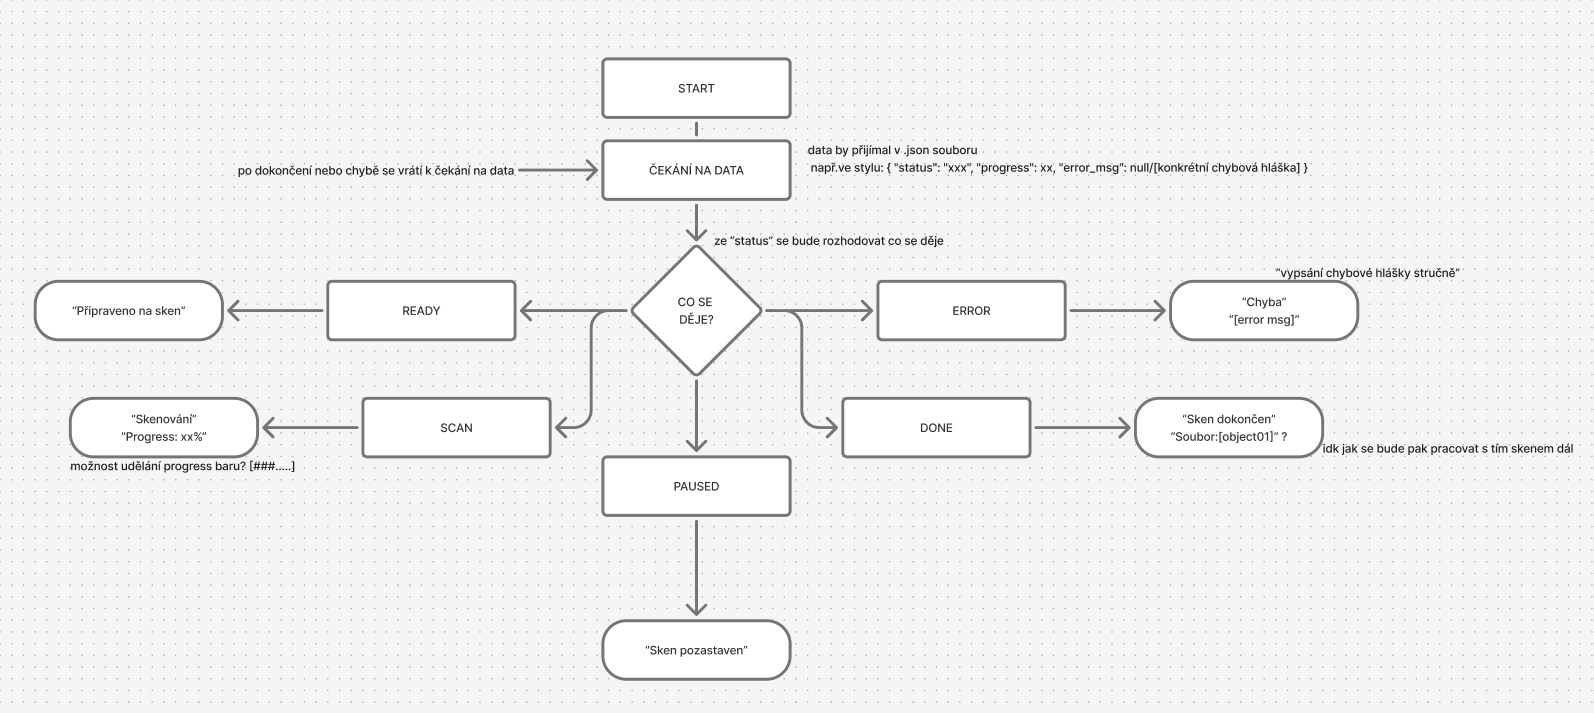
\includegraphics[width=\textwidth]{img/displej_diagram.png}
    \caption{Diagram stavové logiky informačního displeje}
    \label{fig:displej_diagram}
\end{figure}

Mezi definované stavy patří:
\begin{itemize}
    \item \textbf{READY:} Systém je připraven, na displeji svítí text „Připraveno na sken“.
    \item \textbf{SCAN:} Probíhá aktivní snímání. Horní řádek zobrazuje „Skenování“, spodní pak numerický progress bar.
    \item \textbf{PAUSED:} Skenování bylo uživatelem pozastaveno.
    \item \textbf{DONE:} Úspěšné dokončení operace s informací o uloženém souboru.
    \item \textbf{ERROR:} V případě selhání (např. ztráta spojení s kamerou) se vypíše stručná chybová hláška.
\end{itemize}

Po dokončení úlohy nebo odstranění chyby se systém automaticky vrací do stavu čekání na nová data.
\chapter{Závěr a zhodnocení}

\begin{thebibliography}{9}
\bibitem{instructables} 
XIAO, Michael. \textit{Raspberry Pi Laser Scanner} [online]. Instructables, 2020 [cit. 2026-04-29]. Dostupné z: https://www.instructables.com/Raspberry-Pi-Laser-Scanner/
\end{thebibliography}

\end{document}